\section{Desarrollo}
% Metodologia / Desarrollo

\subsection{Generación de la Población Inicial}
La población inicial se generará aleatoriamente, buscando que ningun individuo tenga una aptitud mayor al 0.9,
para poder tener una mejor apreciacion del cambio segun la generación, creando un conjunto de cromosomas binarios de 6 bits. 
Cada cromosoma representará un individuo en la población y se generará de la siguiente manera:

\begin{itemize}
    \item Se crearán 10 individuos (cromosomas) en la población inicial.
    \item Cada cromosoma será una cadena de 6 bits, donde cada bit puede ser 0 o 1.
\end{itemize}

La generación aleatoria de la población inicial es crucial para garantizar la diversidad genética y permitir 
que el algoritmo explore una amplia variedad de soluciones en el espacio de búsqueda.

\begin{figure} [H]
    \centering
    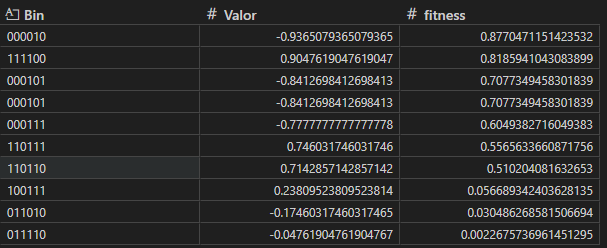
\includegraphics[width=0.65\textwidth]{C:/Users/death/Documents/Maestria/MCIA/Semestre_2/Metaheuristica/Reportes/Alg_Gen/rsc/img/Des/Init_pob.png}
    \caption{Población Inicial ordenada de manera descendente según su aptitud}\label{PoblacionInicial}
\end{figure}

\subsection{Selección}

Con nuestros 10 individuos iniciales, se procederá a seleccionar los padres que participarán en la reproducción para generar
la siguiente generación. Para esto haremos 5 parejas y cada una generará 2 hijos, para mantener el tamaño de la población constante en 10 individuos.

Separaremos la selección en dos grupos de padres según su aptitud, un grupo será el 40\% de los individuos con mayor aptitud y el otro grupo será el 60\% restante.
Para el primer grupo utilizaremos selección por rank (Las que tienen mejor aptitud) y el segundo grupo por torneo (Con peor aptitud esperando que mejoren)

\begin{figure} [H]
    \centering
    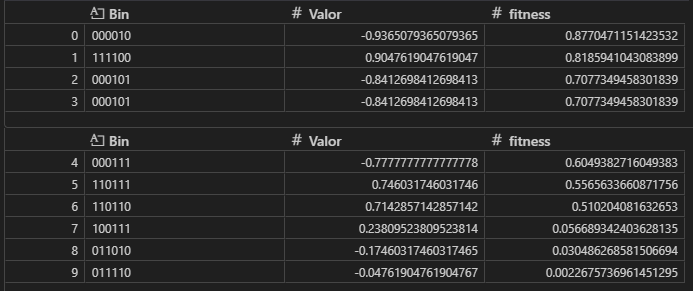
\includegraphics[width=0.65\textwidth]{C:/Users/death/Documents/Maestria/MCIA/Semestre_2/Metaheuristica/Reportes/Alg_Gen/rsc/img/Des/Grupos_padres.png}
    \caption{Grupos de padres por cruza rank (superior) y torneo (inferior)}\label{Selec}
\end{figure}

\subsubsection{Rank}
Para la selección por rank, se ordenan los individuos según su aptitud y se hacen parejas según su rango de aptitud tomando así:  
$(1 - 2), (3 - 4), (5 - 6)\dots(n-1, n)$

Con esto tendremos el siguiente resultado segun nuestro grupo de padres:
\begin{figure} [H]
    \centering
    \includegraphics[width=0.25\textwidth]{C:/Users/death/Documents/Maestria/MCIA/Semestre_2/Metaheuristica/Reportes/Alg_Gen/rsc/img/Des/Rank.png}
    \caption{Padres e hijos generados por cruza rank}\label{Rank}
\end{figure}

Con lo anterior entre padres e hijos, tenemos la siguiente población:
\begin{figure} [H]
    \centering
    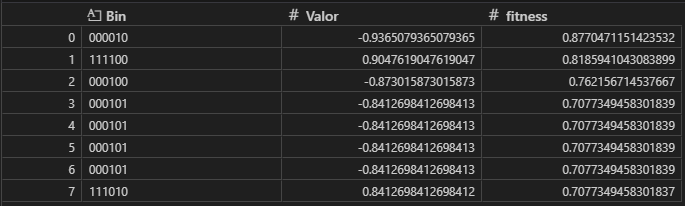
\includegraphics[width=0.65\textwidth]{C:/Users/death/Documents/Maestria/MCIA/Semestre_2/Metaheuristica/Reportes/Alg_Gen/rsc/img/Des/rank_gen.png}
    \caption{Población generada por cruza rank}\label{Pob_rank}
\end{figure}

\subsubsection{Torneo}
Para la selección por torneo, En una lista de n elementos formaremos parejas la siguiente manera:  
$(1 - n), (2 - n-1), (3 - n-2) \dots (n/2 - n/2 + 1)$
Con esto tendremos el siguiente resultado segun nuestro grupo de padres:

\begin{figure} [H]
    \centering
    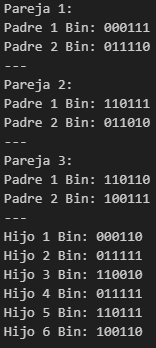
\includegraphics[width=0.25\textwidth]{C:/Users/death/Documents/Maestria/MCIA/Semestre_2/Metaheuristica/Reportes/Alg_Gen/rsc/img/Des/tournament.png}
    \caption{Padres e hijos generados por cruza torneo}\label{Torneo}
\end{figure}

Con lo anterior entre padres e hijos, tenemos la siguiente población:
\begin{figure} [H]  
    \centering
    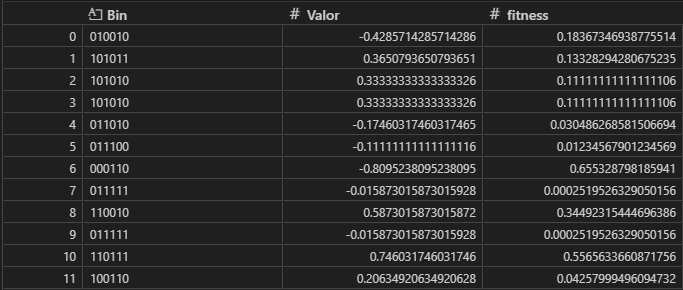
\includegraphics[width=0.65\textwidth]{C:/Users/death/Documents/Maestria/MCIA/Semestre_2/Metaheuristica/Reportes/Alg_Gen/rsc/img/Des/tk_gen.png}
    \caption{Población generada por cruza torneo}\label{Pob_torneo}
\end{figure}

\subsubsection{Seleccion de individuos para la siguiente generación}
Con todo lo anterior tenemos una población de 20 individuos (10 por cada tipo de cruza), por lo que debemos seleccionar los 10 mejores
individuos para formar la siguiente generación, para esto ordenaremos la población de manera descendente según su aptitud y tomaremos 
los primeros 10 individuos.

\begin{figure} [H]
    \centering
    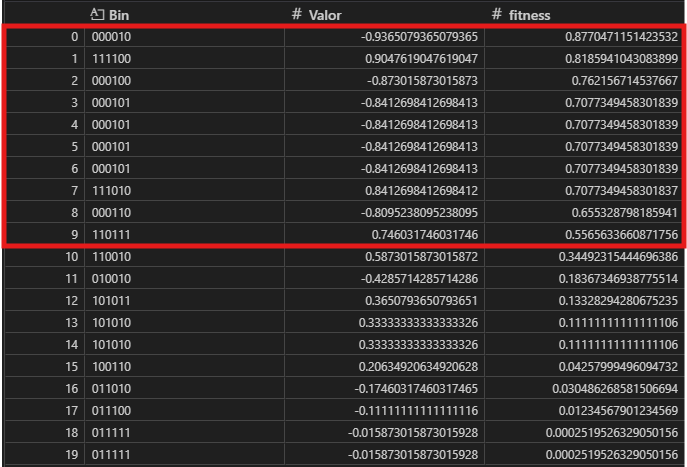
\includegraphics[width=0.65\textwidth]{C:/Users/death/Documents/Maestria/MCIA/Semestre_2/Metaheuristica/Reportes/Alg_Gen/rsc/img/Des/gen1.png}
    \caption{Población seleccionada para la siguiente generación}\label{Pob_selec}
\end{figure}

\subsection{Cruzamiento}
Para el cruzamiento se utilizo el método de un punto, donde se selecciona un punto de corte en los cromosomas de los padres y se intercambian las partes posteriores a ese punto.
Esto permitirá combinar las características de ambos padres en la descendencia, promoviendo la diversidad genética en la población.
En este caso, se seleccionó el punto de corte en la mitad del cromosoma (después del tercer bit) y de esta manera se generaron los hijos de cada pareja de padres.

En este caso no se aplicó mutación, ya que se buscaba observar el comportamiento del algoritmo genético sin la influencia de cambios aleatorios en los individuos.
Por lo que una vez hecho la primera generación, se repitió el proceso de selección y cruzamiento para generar nuevas generaciones de manera iterativa.
Este proceso se repitió durante 5 generaciones más, observando cómo la aptitud de los individuos mejoraba con el tiempo a medida que se seleccionaban y cruzaban los mejores padres.

Con lo anterior mencionado, destacamos que el criterio de paro fue alcanzar un número máximo de generaciones, en este caso 6 generaciones en total (1 inicial + 5 iteraciones).

\subsection{Analisis del Algoritmo Genético}

Despues de completar las 6 generaciones, se observa una mejora significativa en la aptitud de los individuos a lo largo de las generaciones.
La aptitud máxima alcanzada en la última generación es 0.87, lo que indica que el algoritmo ha logrado encontrar soluciones cercanas al óptimo en el espacio de búsqueda definido.
Además, la diversidad genética se ha mantenido a lo largo de las generaciones, con una variedad de individuos presentes en la población final.

Esto se puede apreciar en el siguiente gráfico que muestra la evolución de la aptitud máxima y promedio a lo largo de las generaciones:
\begin{figure} [H]
    \centering
    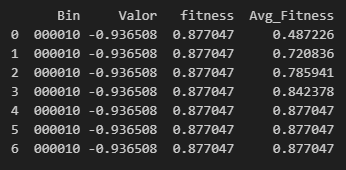
\includegraphics[width=0.5\textwidth]{C:/Users/death/Documents/Maestria/MCIA/Semestre_2/Metaheuristica/Reportes/Alg_Gen/rsc/img/Des/gen_f.png}
    \caption{Mejor población final de 6 generaciones}\label{Gen_final}
\end{figure}
\begin{figure} [H]
    \centering
    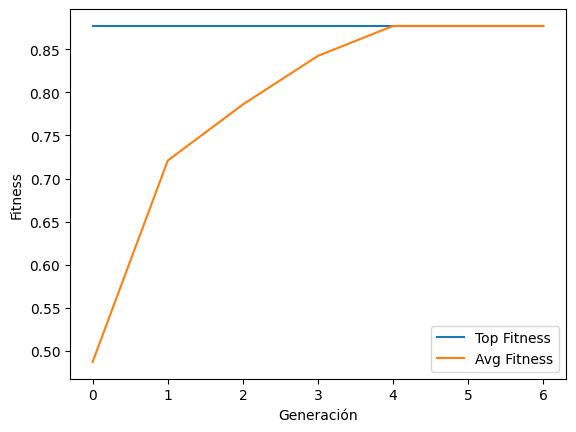
\includegraphics[width=0.75\textwidth]{C:/Users/death/Documents/Maestria/MCIA/Semestre_2/Metaheuristica/Reportes/Alg_Gen/rsc/img/Des/grafica.png}
    \caption{Evolución de la aptitud máxima y promedio a lo largo de las generaciones}\label{Grafica}
\end{figure}

aparte de esto graficamos la aptitud en nuestra funcion objetivo $f(x) = x^2$ para observar como se comporta la aptitud de los individuos en cada generación.

\begin{figure} [H]
    \centering
    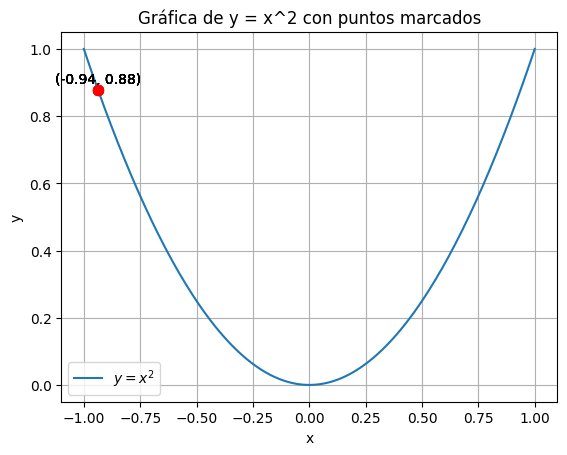
\includegraphics[width=0.75\textwidth]{C:/Users/death/Documents/Maestria/MCIA/Semestre_2/Metaheuristica/Reportes/Alg_Gen/rsc/img/Des/aptitud.png}
    \caption{Evolución de la aptitud en la función objetivo $f(x) = x^2$}\label{Grafica_fitness}
\end{figure}

En resumen, el algoritmo genético ha demostrado ser efectivo para optimizar la función objetivo $f(x) = x^2$ dentro del espacio de búsqueda definido.

\subsection{Segundo Metodo de cruce}
Para observar el comportamiento del algoritmo genético con otro método de cruce, se implementó el cruzamiento de dos puntos. En este método, se seleccionan 
dos puntos de corte en los cromosomas de los padres y se intercambian las partes entre esos puntos. Esto permite una mayor variabilidad en la descendencia y 
puede ayudar a explorar mejor el espacio de búsqueda.

La unica diferencia en la implementación fue el método de cruzamiento, manteniendo el resto del proceso igual, incluyendo la selección por rank y torneo,
así como el criterio de paro basado en un número máximo de generaciones (6 en total). Por lo que se repitió el mismo procreso de selección, cruzamiento y selección de individuos
para generar nuevas generaciones de manera iterativa.

Entonces nos enfocaremos en mostrar el resultado final de la población después de las 6 generaciones, así como la evolución de la aptitud máxima y promedio 
a lo largo de las generaciones.

\begin{figure} [H]
    \centering
    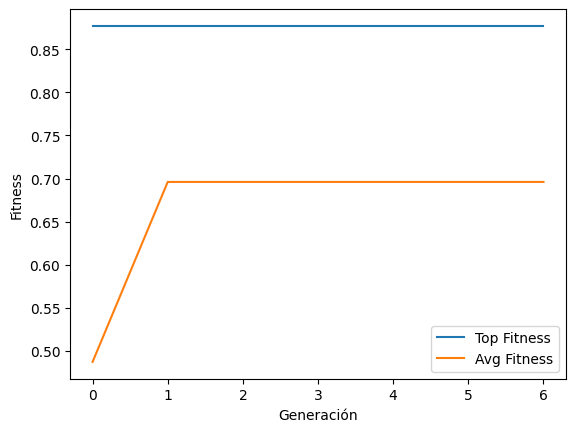
\includegraphics[width=0.65\textwidth]{C:/Users/death/Documents/Maestria/MCIA/Semestre_2/Metaheuristica/Reportes/Alg_Gen/rsc/img/Des/gen2.png}
    \caption{Población final después de 6 generaciones con cruzamiento de dos puntos}\label{Pob_final_2ptos}
\end{figure}